\chapter{Introduction}

This capstone consists of two parts.
The first part is a network science library, \textit{NeTS},
which was created using TypeScript and Deno.
A library, here, refers to code written modularly in such a way that it can be imported and used elsewhere.
Libraries help programmers avoid doing work that was already done by someone else.
Libraries are very important, and make up essential parts of any software project.
NeTS, specifically, can be used for research that relates to network science,
or be imported into other programs or projects to serve as a base for any
kind of computation that involves graphs.
NumPy is an example of an important Python library widely used by programers.
It assists those who use Python with dealing with more complex data structures,
and contains may built-in math functions that make may computations simpler.

Graph Theory is an entire field of mathematics dedicated to studying graphs.
Graphs are a very specific kind of mathematical structure,
that will be formally explained later on.
But, on a most fundamental level, graph theory is about connections.
Network Science is a field that applies the many ideas of Graph Theory to the real world
by giving meaning to the connections it studies.
Most things that involve conections and links,
can be analyzed thruogh the lenses of Network science.
From road networks, to internet architecture, to subway systems, exchange markets, and even organ donations.

The second part of this capstone is this document. It is organized as follows:

Here, in the introduction, the technologies used in the creation of the library are described.
A brief introduction to graph theory is also given.
More complex concepts that relate to network science will also be
provided in later chapters as they become relevant.

In the Types and Interfaces chapter of this document, we give an overview of all the fundamental
data structures and definitions of the library.
After that, the chapter for Values and Functions describes simpler algorithms
of NeTS, and also provides background on these algorithms can be applied through network science.
We will then explain the library's more complex algorithms as well as some of the
decisions that went into writing them the way they currently are.

Lastly, we list further improvements and extensions that could be done with the library.

NeTS is created following its older version, written in the JavaScript (JS) programming language.
That version, Net20, was originally coded for the Spring 2020 Network Science class
at Soka University of America.
Net20 had many flaws and inefficiencies which are addressed by the NeTS library.

NeTS does not have a visualization tool as of the writing of this document.
All images shown here were created using Net20 unless stated otherwise.

\section{Technical Aspects}

JavaScript (JS) is a multi-paradigm programming language.
It is the most-used language in the web.
ECMAScript (ES) is the standardized specification of JS.
ES is updated almost every year and brings many different functionalities to the language, some of which are used in this library.
The latest version of ES is ES2021 (also called ES21),
and is already implemented in most modern browsers.

Typescript (TS) is a strongly-typed programming language that builds on JS.
NeTS is made specifically for dealing with networks,
which are a special kind of mathematical object with very well defined properties.
Thus, TS's type functionality serves the purpose of modeling networks very well.

\section{Basic Graph Theory}

Graph theory is a field of mathematics that studies graphs.
A graph, also called a network, consists of two sets:

1. $V$, a set of vertices (also called nodes), and

2. $E$, a set of edges (also called links)

An edge is a two-element set that cointains two elements from $V$.
Formally, we can write that as:
$$E\subseteq \{\{x,y\}\mid x,y\in V, x\ne y\}$$

Thus, a graph $G$ can be represented as $G=(V,E)$.

\begin{figure}[H]
  \centering
    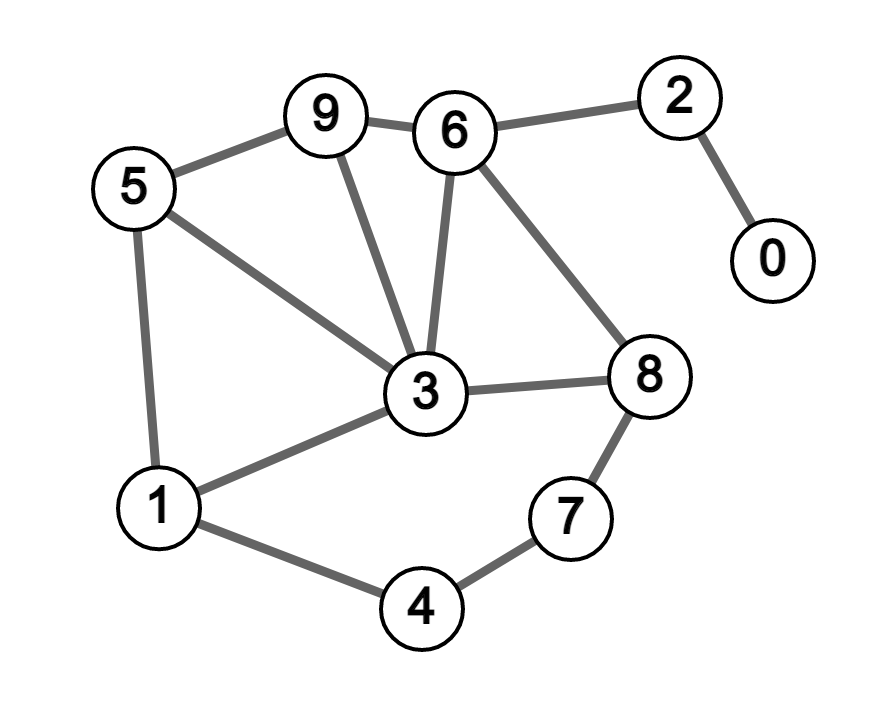
\includegraphics[scale=.25]{img/undirected_sample.png}
    \caption{Example of an undirected network.}
    \label{fig:net_un}
\end{figure}

Graphs are usually defined by the types of edges it can have.
Some of the ways in which we can classify graphs are:
\begin{enumerate}
  \item Directed or undirected: This means an edge can have a direction associated with it.
  A directed network contains edges that are directed from one node to another.
  NeTS deals with both directed and undirected networks.
  A directed network could be used to represent a road network,
  where the roads are represented by edges, and intersections are the vertices.
  An undirected network could be used to represent friendships in a college campus,
  where the edges reflect whether two people are friends or not,
  and the nodes represent the students.
  A common use for network science is the analysis of social networks.
  With a social network, each user is usually represented as a node in the network.
  Edges can be used to express connections: follows, interactions, friendships.
  A specific example of an undirected network is Facebook.
  Users can either be friends or not.
  In contrast to that binary relationship of Facebook friendships,
  we can observe Twitter's system of followers.
  Twitter's network can be represented as a directed graph.
  The connections between users are directional:
  User $A$ can follow user $B$ without the latter following the former.

  \begin{figure}[H]
    \centering
    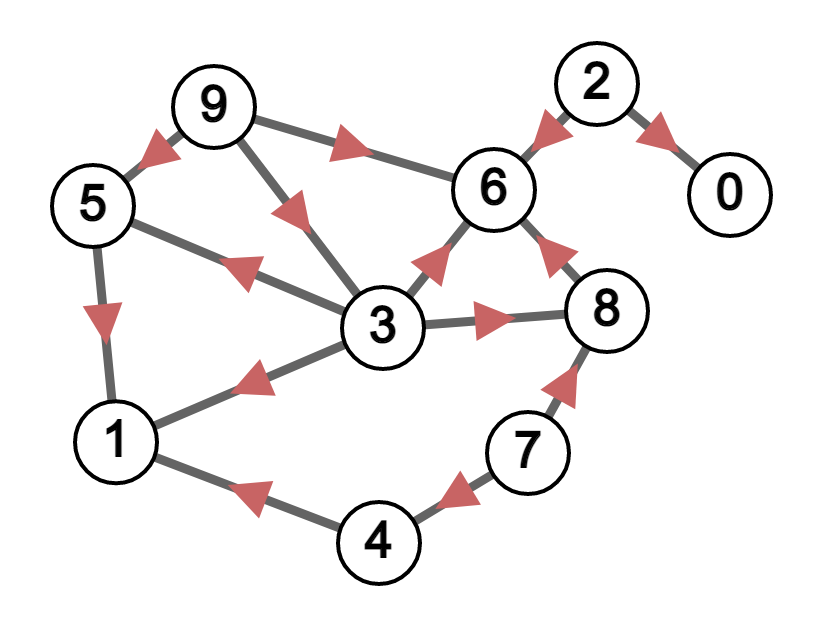
\includegraphics[scale=.25]{img/directed_sample.png}
    \caption{Network in previous example with randomized directed edges.}
    \label{fig:net_di}
  \end{figure}

  \item Self-loops: Networks can also have self-loops, meaning for an edge $e=\{x,y\}$, $x=y$.
  Self-loops are used in state-machines.
  \item Multigraph: Networks can be classified as multigraphs,
  meaning for $e_1,e_2\in E$, $e_1$ and $e_2$
  have the same nodes, but represent different edges. Back to the road network example, a two-way street that connects two
  intersections could be represented as two different edges that connect the same two nodes.
  \item Simple graph: simple graphs are undirected graphs with no self-loops, and no multiple edges.
  NeTS only deals simple graphs.
  Nevertheless, there are some functions that are setup with compatibility with
  multigraphs in mind. Thus, although multigraphs are beyond the scope of this capstone,
  in the future, NeTS could be adapted to work with multigraphs.
  \item Weighted or Unweighted: Traditionally, a weighted network means the edges in the network are weighted.
  However, it is also possible to weight vertices.
  Continuing with the example of social networks,
  we can take a look at Facebook's Messenger.
  An edge between two nodes (users) could represent
  whether they have ever sent messages to each other,
  while the number of messeges exchanged could
  be represented by the edge's weight.
  A vertex's weight, on the other hand,
  could help represent the GDP of countries in a
  network of global trade where an edge between
  two countries represents if they trade.
  The library considers all networks to be weighted on a technical level.
  This means that, when created, any edge or vertex has their weight set to 1.
  An unweighted network is thus just a network with all weights set to the default of 1.
  Visually, the weight of an edge is usually represented as thickness.
\end{enumerate}

\begin{figure}[H]
  \centering
  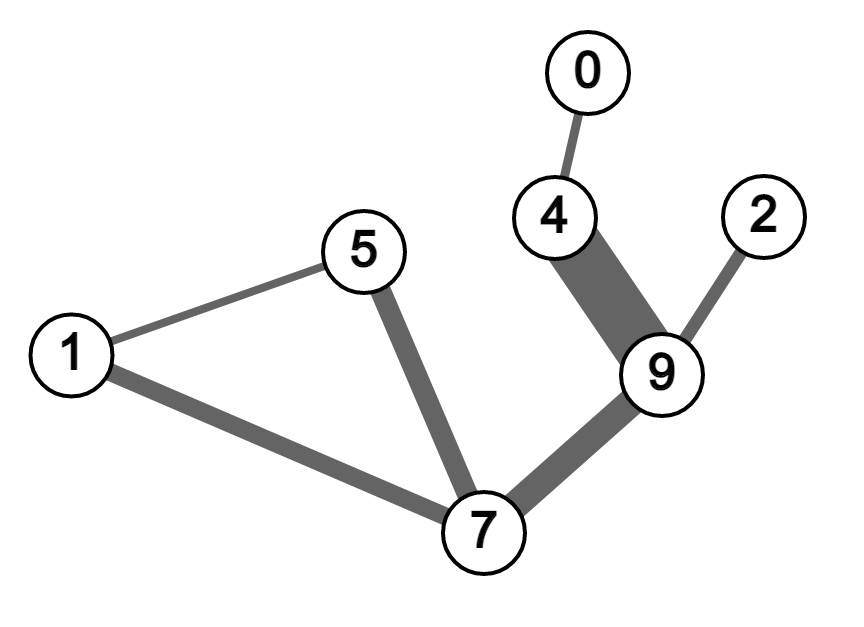
\includegraphics[scale=.25]{img/weighted_sample.png}
  \caption{A network with weighted edges. In the example of Messenger,
          we could say that $5$ and $4$ have never message each other,
          while $4$ and $9$ have exchanged many messages.}
  \label{fig:net_weight}
\end{figure}